\documentclass[11pt,a4paper]{article}
\usepackage[utf8]{inputenc}
\usepackage{amsmath}
\usepackage{amsfonts}
\usepackage{amssymb}
\usepackage{graphicx}
\usepackage{csquotes}% Recommended
\usepackage[toc, nonumberlist, acronym]{glossaries}
\usepackage{multirow}
\usepackage{float}
\usepackage{eurosym}
\usepackage[ngerman]{babel}
\usepackage{longtable}
\usepackage{pdfpages}

\usepackage[style=authoryear-ibid,backend=biber]{biblatex}

\addbibresource{main.bib}

\author{Pia Erbrath}
\title{Tools to Sign Documents Electronically - a Research}
\makeglossaries

\begin{document}
	\maketitle
	\pagenumbering{Roman}
	\tableofcontents
	\listoftables
	\newpage
	\newglossaryentry{eidas}{name={eIDAS},description={Regulation from European  parliament and council regarding electronic identification and trust services for  electronic  transactions  in  the  internal  market  and repealing  Directive  1999/93/EC}}
\newglossaryentry{gdpr}{name={GDPR},description={General Data Protection Regulation \newline}}


\newacronym{cc}{cc}{codecentric AG}
\newacronym{os}{OS}{operating system}
\newacronym{api}{API}{Appliaction Programming Interface}
\newacronym{sdk}{SDK}{Software Development Kit}
\newacronym{eu}{EU}{European Union}
\newacronym{pdf}{PDF}{Portable Document Format}
\newacronym{es}{ES}{Electronic signature}
\newacronym{erp}{erp}{Enterprise Resource Planning}
\newacronym{bs}{BS}{biometric signature}
\newacronym{app}{App}{application}
\newacronym{aes}{AES}{advanced electronic signature}
\newacronym{mb}{MB}{Mega Byte}
\newacronym{eidas}{eIDAS}{eIDAS}
\newacronym{usa}{USA}{United States of America}
\newacronym{os}{OS}{operating system}
\newacronym{saas}{SaaS}{Software as a Service}
\newacronym{op}{OP}{On-Premise}
\newacronym{ses}{SES}{simple electronic signature}
\newacronym{qes}{QES}{qualified electronic signature}
\newacronym{sms}{SMS}{Shoet Message Service}

\printglossaries
	\clearpage
	\pagenumbering{arabic}
	\section{Introduction}

At codecentric AG a paperless office should be introduced. That means all contracts and offers possible should be signed and achieved in digitally way. Currently for some contracts a tool is used to sign documents digital, but that should be extended. Also, the achieving is done digital, but in a manual way with scanning of the signed documents and then uploading them to the achieve. Inside this research the topic of \gls{es} is covered, which is part of the paperless office.

This research contains the following aspects of a research: First the scope of the research is described, then the questions which will be answered in this research and how they are answered will be explained. Next the criteria and the weight of them are described to can advice which signature should be used later, followed by presenting the results of the research and a comparison of the different kinds of signatures. Finally, an advice is given.  
	\section{Scope}
The scope of this research is to figure out which tool for electronic document signing fits best the requirements given from the company \gls{cc}. Due to the fact that there are many tools available only a selection is done. From the company the tools \textit{HelloSign} and \textit{DocuSign}, solution from partner companies and the solution from the company \textit{Wacom} should be taken into account. Additionally, other tools will be taken into account, but this is only a selection based on an internet research. How this is been done, is explained in the next section.



	\section{Questions}

In this research the question will be answered which available tool or technology fits best the requirements of \gls{cc} to sign documents electronically to work more efficient. The  question will be answered through an internet research. Tools will be selected based on the information of different comparison portals and the information provided by the company itself. Furthermore, there will be some testing of the functionalities if possible to prove the usability for \gls{cc}. 

For the testing of the functional requirements like order of singing and the simple usage the preset up is to creation of three test mail addresses and three documents of the format \gls{pdf}, Microsoft word and Open Office writer. The real testing is based on the following steps:
\begin{enumerate}
	\item Register with master mail address to the tool.
	\item Upload the document.
	\item Enter other mail address to sign document.
	\item Select order of signing if possible.
	\item Add fields to sign if needed.
	\item Sign document with master mail address.
	\item Release document for other mail addresses.
	\item Do one of those steps:
	\begin{enumerate}
		\item Try to sign against order.
		\item Try to decline of document signing.
		\item Sign document with unknown account.
		\item Sign document with known accountt. 
	\end{enumerate}
	\item Check current state of the process.
	\item In the case the document is signed by all, check the availability of the document and download it.
\end{enumerate}
	\section{Criteria \& Weightings} \label{tool:sec:criteria}
Inside this section the different criteria are explained and divided in their
weighted categories. The criteria are the following:
\begin{itemize}
	\item Integration \newline
	Weight: 8 \newline
		The most important criterion is the integration, because the tool should be interact with the \gls{erp} and the Google Suite used by \gls{cc}. In the best case all the tools can be used in one system. This means they are in such a way integrated with each other, that the end user do not need to switch the applications. \newline
		This criterion is a knockout criterion. In the case it is not fulfilled the tool will be automatically ignored for the process realization. 
	\item Device independent \newline
	Weight: 7 \newline
	Due to the fact that all employees of \gls{cc} have different \gls{os} for their computer and smart phones, should be the tool hardware independent. Furthermore, it is stated that the employees and execution board is not always at the buildings of the company available, doing home office or working by the customers. This leads to the preference of having \gls{app} for the tool, so that the employees of \gls{cc} can sign the documents everywhere they are independent of their device available.\newline
	This criterion is a knockout criterion. In the case it is not fulfilled the tool will be automatically ignored for the process realization. 
	\item Usability \newline
	Weight: 6 \newline
	Another requirement is the usability. For the reason that several employees should use the tool, it need to be simple to use. There should be no long learning time and the handling need be intuitive or at least the tool should provide information about buttons or next steps. In the best case the tool has a lot of automated processes, so that the user do not care about what to add where and with which information.
	\item Costs \newline
	Weight: 5 \newline
	It is important to have the costs in focus. If they are too high the cost-benefit ratio will be negative and the effect of the new process for \gls{cc} is non existing. The areas pricing model, access to functionalities and amount of accounts fall into this category. For this research price information for 2.400 documents and 80 users should be collected and then calculate this price for one document to get information about the price per document. The classification should be done based on the average of all tools taken into account.
	\item Accepted file formats \newline
	Weight: 4 \newline
	\Gls{cc} uses in general three different file formats for their documents. It should with the tool possible to use them in the future with the tool to sign the documents without converting them into another format.
	\item Operating mode \newline
	Weight: 3 \newline
	Another criterion is the operating mode. That means runs the tool as \gls{saas} or \gls{op}, need \gls{cc} provide its own server and need to care about its security and backup or does the provider of the tool offers this within his plan. This influence also the costs of the tool.
	\item Additional security \newline
	Weight: 2 \newline
	To be sure that the correct person use the service and to increase the security, \gls{cc} uses the Two-Factor authentication for most systems and tools they use. This should be also available for the signature tool.
	\item Legal aspects \newline
	Weight: 1 \newline
	The tool should satisfy certain legal standards, so that \gls{cc} could be use the signing as evidence. This is also important in respect to further use cases for the tool at \gls{cc}, where a higher standard exist than for quotations.
\end{itemize}

The table \ref{tool:tab:resTcateg} displays the different categories for each criterion and shows
their weighting. The best weighting is (+ +) and the worst is (- -). 

%\begin{table}[h!]
	\begin{longtable}{|p{4cm}|p{9cm}|p{1.5cm}|} \hline
		\rowcolor{Gray}Criterion & Category & Weighting \\ \hline
		\multirow{6}{*}{Integration} & No & - - \\ \cline{2-3}
									& Tools for workflow building & o \\ \cline{2-3}
									& Predefined integrations for some tools at \gls{cc} exists already & o \\ \cline{2-3}
									& \Gls{api} and/or \gls{sdk} & + \\ \cline{2-3}
									& \Gls{api} and/or \gls{sdk} \& predefined integrations for some tools that are already in usage & + + \\ \cline{2-3}
									& Predefined integrations for all tools used at \gls{cc} & + + \\ \hline 
		\multirow{8}{*}{Device independent} & Additional hardware required & - - \\ \cline{2-3}
											& Only for certain \gls{os} for Desktop & - - \\ \cline{2-3}
											& Only for certain \gls{os} for smart phone & - - \\ \cline{2-3} 
											& Only for Desktop & - \\ \cline{2-3}
											& Only for smart phone & o \\ \cline{2-3}
											& Only for programmed devices & o \\ \cline{2-3}
											& Only web application & + \\ \cline{2-3}
											& With web application and for all \gls{os} of smart phone and Desktop & + + \\ \hline
		\multirow{5}{*}{Usability} & A lot of actions to set required fields \& activate sharing & - - \\ \cline{2-3}
								    & A few actions to set required fields \& activate sharing & o \\ \cline{2-3}
									& A few actions to set required fields \& activate sharing \& company stamp can be recorded & + \\ \cline{2-3}
									& Recognize where to set fields & + \\ \cline{2-3}
									& Recognize where to set fields \& company stamp can be recorded & + + \\ \hline
		\multirow{5}{*}{Costs}  & $ \textgreater +25\% \varnothing $ & - - \\ \cline{2-3}
								& $ \textgreater \varnothing \& \leq +25\% \varnothing $ & - \\ \cline{2-3}
								& $ \textgreater -25\% \varnothing \& \leq \varnothing  $ & o \\ \cline{2-3}
								& $ \textgreater -50\% \varnothing \& \leq -25\% \varnothing $ & + \\ \cline{2-3}
								& $ \leq -50\% \varnothing $ & + + \\ \hline
		\multirow{4}{*}{Accepted file formats} & Special type & - - \\ \cline{2-3}
												& \Gls{PDF} & o \\ \cline{2-3}
												& \Gls{PDF} \& Microsoft Word (doc, docx) & + \\ \cline{2-3}
												& \Gls{PDF}, Microsoft Word \& Open Office Writer(odt) & + + \\ \hline
		\multirow{2}{*}{Operating mode} & \gls{op} & o \\ \cline{2-3}
										 & \gls{saas} & + + \\ \hline
		\multirow{6}{*}{Additional security} & None & - - \\ \cline{2-3}
											& Question and Answer & o \\ \cline{2-3} 
											& Online identity & o \\ \cline{2-3}
											& Authentication with mobile phone & + \\ \cline{2-3}
											& Authentication with video, personal ID or similar & + + \\ \cline{2-3}
											& Certification & + + \\ \hline
		\multirow{6}{*}{Legal aspects} & No & - - \\ \cline{2-3}
										& \gls{eidas} fulfilled with \gls{ses} & - \\ \cline{2-3}
										& \gls{eidas} \& \glossary{gdpr} fulfilled with \gls{ses} & o \\ \cline{2-3}
										& \gls{eidas} \& \glossary{gdpr} fulfilled with \gls{aes} or \gls{qes} & + \\ \cline{2-3}
										& \gls{eidas} \& \glossary{gdpr} fulfilled with \gls{aes} or \gls{qes} \& global accepted & + + \\ \hline
	\caption{Categories and their weighings}
	\label{tool:tab:resTcateg}
	\end{longtable}
%	\caption{Categories and their weighings}
%	\label{tab:resTcateg}
%\end{table}
%\newpage
	\section{Result}
In this section different tools will be described, their test result presented and the general information of them summarized.

\subsection{Wacom sign pro PDF}
This tool is provided by the company Wacom, which is the customer previously thought for the bachelor project. At the moment there is an \gls{app} available, that signs documents with a \gls{bs} \parencite{wacom2018pdf}. Currently Wacom develops an \gls{sdk} based on the \gls{app}, therefore is no testing possible. The information presented in table \ref{tab:wacom} are from the internet and a product presentation from first March 2018 at the Wacom site in Düsseldorf. 
\begin{table}[h]
	\begin{tabular}{|p{4cm}|p{10cm}|} \hline
		Criterion & Fulfillment \\ \hline
		Usage without license & At the moment not clear. The \gls{app} currently has a free version, but with limited usage.\\ \hline
		Devices independent & The usage of this technology requires hardware at the moment. Therefore, several options exist. Either you have a smart phone with a pen, an iOS phone, a Windows computer with touch recognition or a Windows computer with additional hardware.\\ \hline
		Integration possible & This year a new \gls{sdk} will be published that allows the integration with existing tools. \\ \hline
		Certified & The software uses the \gls{bs} and \gls{aes}. Currently there is no defined status by the government for the \gls{bs}. But in combination with the \gls{aes} it has a legal status. \\ \hline
		Easy usage & Select field(s) to enter data and sign with the pen, press button to agree and then enter mail to sharing. It is not described if a company stamp could be inserted.\\ \hline
		Costs & Unclear, due to the fact that the \gls{sdk} is not published and no pricing is published.\\ \hline
		Accepted documents & \Gls{pdf}\\ \hline
		Amount of accounts & At the moment also unclear due to the fact that the usage requirements are not published. The \gls{app} currently allows more than 5000 in one environment. \\ \hline
	\end{tabular}
	\caption{Summary Wacom sign pro PDF}
	\label{tab:wacom}
\end{table}

\subsection{DocuSign}
This tool is already in usage at \gls{cc}, but not always and with a lot of manual actions and missing things like the company stamp. During the testing a lot of functionalities were figured out. The test protocol is placed in the appendix \ref{sec:docusign}. The table \ref{tab:docusign} below will give a short summary about the test result and other aspects figured out during the research.

\begin{table}[h]
	\begin{tabular}{|p{4cm}|p{10cm}|} \hline
		Criterion & Fulfillment \\ \hline
		Usage without license & Yes, just need to add some information required from the person request the signing like name and mail address for signing. In the case of uploading and managing the documents an account is required.\\ \hline
		Devices independent & Online available, also a \gls{app} is accessible for all \gls{os} of smartphones \parencite{docusign2018mobile}. \\ \hline
		Integration possible & A \gls{sdk} available within the \grqq Business Flex\grqq packet of the provider. Also an integration is possible with Google Drive, but therefore the Google Drive cloud need to be connected to DocuSign \parencite{docusign2018integration,docusign2018formats}. \\ \hline
		Certified & DocuSign satisfies the standards of the \gls{eidas} and more security standards \parencite{docusign2018certificates,docusign2018legal}. \\ \hline
		Easy usage & The fields need to be set manual, it need to be checked if it possible to customize it. Furthermore it is possible to track activities, assign signer, add the company stamp, transfer the signing responsibility, decline the signing and to sign the document manual and scan it then. \\ \hline
		Costs & The provider of DocuSign offers different plans. \Gls{cc} needs at least the \textit{Business Pro} Plan for one user, which costs 480\$ per year, and the \textit{intermediate API} plan with 3420\$ per year. But due to the fact, that there will  e more than one user, the enterprise offerings should be requested. \parencite{docusign2018api,docusign2018user} \\ \hline
		Accepted documents & PDF \& Microsoft Word accepted, Open Office Writer is not accepted. Moreover, the maximum accepted size of a document is 25 \gls{mb}. \parencite{docusign2018formats} \\ \hline
		Amount of accounts & Depending on the license ordered.\\ \hline
	\end{tabular}
	\caption{Summary DocuSign}
	\label{tab:docusign}
\end{table}

\subsection{HelloSign}
The online tool HelloSign is used at the subsidiary company Istana of \gls{cc}. Therefore, it should also taken into account. Not all functionalities could be tested through the fact that for the business version data were requested, the tester was not allowed to give. The result of the test is documented in appendix \ref{sec:hellosign} and a summary of it together with additional information collected from an online research is given in table \ref{tab:hellosign}.
\begin{table}[h]
	\begin{tabular}{|p{4cm}|p{10cm}|} \hline
		Criterion & Fulfillment \\ \hline
		Usage without license & Signing without account possible, but the signed documents could not be viewed online and uploaded if no account exists. It will be send within a mail. Moreover, there is the fact that the free version only allows to send three documents per month. This leads to the result, that a higher version is required \parencite{hellosign2018price}. \\ \hline
		Devices independent & The tool is online available. Furthermore, exists an \gls{app} for Android and iOS, but it has not the same functionalities as the online platform.  \parencite{hellosign2018legal} \\ \hline
		Integration possible & HelloSign has an \gls{api} with different version provided, included there are several functionalities. Moreover, integration exists for Google services like Google Suite and for several other business applications e.g. HubSpot CRM, which used at \gls{cc}. Additionally third party integrations are possible with Zapier, a tool for modeling business processes. \parencite{hellosign2018integration,hellosign2018api} \\ \hline
		Certified & The tool fulfills the requirements of the \gls{eidas} regulations of the \gls{eu} and can be used in the \gls{usa} \parencite{hellosign2018legal} \\ \hline
		Easy usage & It is simple to upload a document and sign it, due to the fact that there is intuitive handling. Not all functionalities like branding and company stamp could be tested, because of the non usable test version of higher plans. The fields required for signing need to be set manual and there is not that much choice of fields. In the case the \gls{app} is used, only the creation of a signing process could be done. \\ \hline
		Costs & For the usage at \gls{cc} two different licenses are required. First the \gls{api} license where at least the version API Gold is need which costs 449\$ per month. The second license is the user license. Therefore the User Business version is required at least with five senders. It costs 40\$ per month. But due to the fact, that more senders are needed the Enterprise version is advisable. Yet the price is not given in the internet\parencite{hellosign2018price,hellosign2018api} .\\ \hline
		Accepted documents & HelloSign accepts several documents format. In the test the formats \gls{pdf}, Microsoft Word and Open Office Writer was accepted. The maximal amount of a pages a document is 500 pages or a file size of 40th \gls{mb} \parencite{hellosign2018documents}. \\ \hline
		Amount of accounts & Inside the business version of HelloSign 5 senders/accounts are involved, for more accounts the provider need to be requested \parencite{hellosign2018price}. \\ \hline
	\end{tabular}
	\caption{Summary HelloSign}
	\label{tab:hellosign}
\end{table}

\subsection{SignDoc}
This tool is provided by Kofax, a partner of \gls{cc}.

\begin{table}[h]
	\begin{tabular}{|p{4cm}|p{10cm}|} \hline
		Criterion & Fulfillment \\ \hline
		Usage without license & \\ \hline
		Devices independent & \\ \hline
		Integration possible & \\ \hline
		Certified & \\ \hline
		Easy usage & \\ \hline
		Costs & \\ \hline
		Accepted documents & \\ \hline
		Amount of accounts & \\ \hline
	\end{tabular}
	\caption{Summary SignDoc}
	\label{tab:signdoc}
\end{table}

\subsection{Adobe Sign}

\begin{table}[h]
	\begin{tabular}{|p{4cm}|p{10cm}|} \hline
		Criterion & Fulfillment \\ \hline
		Usage without license & yes, but for starting license required\\ \hline
		Devices independent & web, app iOS and Android (require certain os version) \\ \hline
		Integration possible & A lot of integration with tools possible, api available \parencite{adobesign2018integration,adobesign2018info} \\ \hline
		Certified & eIdas \parencite{adobesign2018legal} \\ \hline
		Easy usage & \\ \hline
		Costs & Enterprise plan required, but no price published online \parencite{adobesign2018costs} \\ \hline
		Accepted documents & PDF, Microsoft Word \parencite{adobesign2018info} \\ \hline
		Amount of accounts & Unknown \\ \hline
	\end{tabular}
	\caption{Summary Adobe Sign}
	\label{tab:adobesign}
\end{table}

\subsection{SignNow}

\begin{table}[h]
	\begin{tabular}{|p{4cm}|p{10cm}|} \hline
		Criterion & Fulfillment \\ \hline
		Usage without license & \\ \hline
		Devices independent & \\ \hline
		Integration possible & \\ \hline
		Certified & \\ \hline
		Easy usage & \\ \hline
		Costs & \\ \hline
		Accepted documents & \\ \hline
		Amount of accounts & \\ \hline
	\end{tabular}
	\caption{Summary SignNow}
	\label{tab:signnow}
\end{table}

\subsection{RightSignature}

\begin{table}[h]
	\begin{tabular}{|p{4cm}|p{10cm}|} \hline
		Criterion & Fulfillment \\ \hline
		Usage without license & \\ \hline
		Devices independent & \\ \hline
		Integration possible & \\ \hline
		Certified & \\ \hline
		Easy usage & \\ \hline
		Costs & \\ \hline
		Accepted documents & \\ \hline
		Amount of accounts & \\ \hline
	\end{tabular}
	\caption{Summary RightSignature}
	\label{tab:rightsignature}
\end{table}

\subsection{eSign Live}

\begin{table}[h]
	\begin{tabular}{|p{4cm}|p{10cm}|} \hline
		Criterion & Fulfillment \\ \hline
		Usage without license & \\ \hline
		Devices independent & \\ \hline
		Integration possible & \\ \hline
		Certified & \\ \hline
		Easy usage & \\ \hline
		Costs & \\ \hline
		Accepted documents & \\ \hline
		Amount of accounts & \\ \hline
	\end{tabular}
	\caption{Summary eSign Live}
	\label{tab:esign}
\end{table}

\subsection{PandaDoc}

\begin{table}[h]
	\begin{tabular}{|p{4cm}|p{10cm}|} \hline
		Criterion & Fulfillment \\ \hline
		Usage without license & \\ \hline
		Devices independent & \\ \hline
		Integration possible & \\ \hline
		Certified & \\ \hline
		Easy usage & \\ \hline
		Costs & \\ \hline
		Accepted documents & \\ \hline
		Amount of accounts & \\ \hline
	\end{tabular}
	\caption{Summary PandaDoc}
	\label{tab:pandadoc}
\end{table}

\subsection{eSignAnyWhere}

	\section{Comparison} \label{sec:comp}

	\section{Advice}
In general need to be said that \glspl{es} are a good alternative for handwriting signatures, especially in \gls{eu} states. The focus is on the type of \gls{es}. The result from the comparison in section \ref{sec:comp} is that the \gls{qes} fits the requirements explained in section \ref{Tab:criteria} best. Also from the legal aspect would it be the best solution, cause of the fact that it is equated to the written signature in the most cases. Even customers with a high demand on legal aspects will be satisfied with that signature, cause of the possibility to track document changes after the signing and the identification of the signers. 
	\clearpage
	\printbibliography
	\clearpage
	\appendix
	\section{Test Protocol DocuSign}
Inside this part the testing of the tool DocuSign is documented. The tests are executed based on the definitions of research about Tools to Sign Documents Electronically. It is done at the third and fourth April 2018. 

\subsection{Registration}
The registration for testing the tool is simple. The following data need to be added:
\begin{itemize}
	\item Name,
	\item Email,
	\item Job title,
	\item Company,
	\item Business area,
	\item Amount of employees,
	\item Phone number and
	\item A reason why it is used.
\end{itemize}
Later you need to select a password and confirm it. The testing duration will take 30th days. After that time the signed documents are still available, but a new starting of a signing process is not possible without payment. It also possible to sign free, but that is limited through the number of starting a signing process. 

The normal login is simple, you only need to enter your mail and the selected password. That is the same for the \gls{app}. In the case a person only needs sign a document, no registration is necessary. The person can access the document via a link every time.

\subsection{Uploading Documents}
In the web version a button is available which opens by clicking a document chooser with the directory of the computer the web browser is opened. Through that the navigation is similar to other tools like Microsoft Word. Now the tester can navigate to the test document and select it. Then DocuSign offers the option to select additional files. It is also possible to add a document with the drag-and-drop functionality. Furthermore, a document could be chosen from templates stored at DocuSign. If the \gls{app} is used a photo from the document could be made and this could then be used to sign.

In the case a document is selected and uploaded, several actions could be done with it: Show the document, rename it, compare it with a template, replace or delete the document. DocuSign accepts several document types like \gls{pdf} or Microsoft Words .docx.

\subsection{Sharing of Documents}
The sharing is simple. Only the name and the mail address of the person need to sign is to enter. In the case the person was already requested to sign a document, the contact data is stored by DocuSign in the web version and could be selected with the address book. The \gls{app} uses the contact data from the smartphone.
As a feature different roles could be selected:
\begin{enumerate}
	\item A person which need to sign
	\item A person which sign locally (only in the business version)
	\item A person which receives an information
\end{enumerate}
Moreover, there is the option to add an additional security level. This is done by requesting an access code defined by adding the person to sign. In the case the person now want to sign, he/she need to enter before the code. This code need to be transmitted somehow to this person. Furthermore, it is feasible to remove a person from the list of sharing. 

\subsection{Select Order of Signing}
Within the web application it is possible to select an order for the signing, with the test in the \gls{app} it was not possible. It is simple, either do it with drag-and-drop or enter the number before the contact box. Also, the user can select if a order is necessary or if two or more person need to sign first ante the other persons.

\subsection{Preparation for Signing}
In this action all required fields need to be manual placed in the document. This is quite easy and there are a lot of fields type by default, which can be customized in the business version of the tool. The fields are for example signature, name, mail or date of signing.
Also, it is possible to twist the document if it is necessary. Furthermore, there is the option that on each document file uploaded to sign could be prepared separate. 

\subsection{Company Stamp}
The tool allows the using of stamps. Therefore, this option need to be activated in the settings. When this action is done, a new field type is available by the preparation for the signing action.

In the case the stamp is the first time requested, a window is open with the request to upload a picture of the stamp. This picture can be fit and gets a name. Also there is the option to declare the created stamp as default stamp. 

\subsection{Signing Documents}
Within the step of signing a document several options are possible, each of them is described bellow.

\subsubsection{One Person}
Regarding the fact that not always more than one person need to sign, two options exist. First the person who start the process need to sign or second another person need to sign. Both cases are similar and are basically the same as multiple person would sign the document. The only difference is that int he first option the user will be redirected after the preparation to the signing action. int he other case the user receives an mail. 

\subsubsection{Multiple Persons}
All persons get an invitation via mail to sign the document. If there is a specified order, they receive the mail not until the person(s) need to sign previous have signed it successfully. When all persons have signed the document, all of them will receive a mail with the link to the completed document.

\subsubsection{Unregistered Person}
If the person need to sign the document is not registered at DocuSign, he gets an mail and can access the document via a button or link. Then the person need to agree the usage of an \gls{es} or can select other options like decline or alternatives explained in the features. Next the requested fields need to be filled in. In the case of the signature filed, the person can correct the name and the initials and is allowed to choose between selecting a signature style or drawing the signature with the mouse. Finally, if all required fields are filled in, the signing process could be finished, a windows pop ups with the option to register at DocuSign and a mail is send to all parties when the document is completely signed. 

\subsubsection{Decline Signing}
All persons, who not started the signing process, have the right to decline the signing. Then the complete order of signing is stopped and all parties get a mail with the information about the declining. The person have the option to enter a reason, which is also submitted with the mail.

\subsubsection{Features}
The tool provides several features not requested in the test setup, but are still tested. They will be explained beneath.
\paragraph{Signing in a Local Session}
When the mail is received with the link of the to be signed document and the button is clicked to access it, first an information page about the process is shown. After the clicking the start button the users are leaded through the process. The person need to be signed, accept the using of the \gls{es} and can then fill in the fields. In the case of the signature filed, the person can correct the name and the initials and is allowed to choose between selecting a signature style or drawing the signature with the mouse. Finally, if all required fields are filled in, the signing process could be finished, a mail address is requested to send a copy of complete signed document. 

\paragraph{Print and Sign}
Sometimes a person or company accepts the \gls{es}, but want to sign with the handwritten signature. Therefore, this option exists at DocuSign. The person which had to sign can print the document, sign it with all required fields manual and either upload it again to DocuSign or send with fax back.

ToDo testing 

\paragraph{Assign to Someone Else}
Regarding the fact, that not every time the correct person is assigned to sign a document, DocuSign offers the option to redirect this task, by the person which receive the invitation of signing. This person can refer the document to a different person by adding their name and mail address and gets a copy of the signed document. The other person receives a request to sign the document as described above. Every time the document owner, who started the signing process, is informed about such changes.
It is possible to denied such action by setting a permission at the step where the process is started. 

\subsection{Status Report}
Within DocuSign it is possible to track the status of a document. Several different information exist like at which time some received, looked and signed the document. In this functionality other actions could be triggered like sending the document again, make changes to it or download the current document.

Furthermore, there is the options for those users which have a DocuSign account to see open documents, that are assigned to be signed by them. This view also available in the \gls{app}.

\subsection{Availability of Documents}
After the signing process is completed, 
\label{sec:docusign}

\section{Test Protocol DocuSign}
Inside this part the testing of the tool DocuSign is documented. The tests are executed based on the definitions of research about Tools to Sign Documents Electronically. It is done at the third and fourth April 2018. 

\subsection{Registration}
The registration for testing the tool is simple. The following data need to be added:
\begin{itemize}
	\item Name,
	\item Email,
	\item Job title,
	\item Company,
	\item Business area,
	\item Amount of employees,
	\item Phone number and
	\item A reason why it is used.
\end{itemize}
Later you need to select a password and confirm it. The testing duration will take 30th days. After that time the signed documents are still available, but a new starting of a signing process is not possible without payment. It also possible to sign free, but that is limited through the number of starting a signing process. 

The normal login is simple, you only need to enter your mail and the selected password. That is the same for the \gls{app}. In the case a person only needs sign a document, no registration is necessary. The person can access the document via a link every time.

\subsection{Uploading Documents}
In the web version a button is available which opens by clicking a document chooser with the directory of the computer the web browser is opened. Through that the navigation is similar to other tools like Microsoft Word. Now the tester can navigate to the test document and select it. Then DocuSign offers the option to select additional files. It is also possible to add a document with the drag-and-drop functionality. Furthermore, a document could be chosen from templates stored at DocuSign. If the \gls{app} is used a photo from the document could be made and this could then be used to sign.

In the case a document is selected and uploaded, several actions could be done with it: Show the document, rename it, compare it with a template, replace or delete the document. DocuSign accepts several document types like \gls{pdf} or Microsoft Words .docx.

\subsection{Sharing of Documents}
The sharing is simple. Only the name and the mail address of the person need to sign is to enter. In the case the person was already requested to sign a document, the contact data is stored by DocuSign in the web version and could be selected with the address book. The \gls{app} uses the contact data from the smartphone.
As a feature different roles could be selected:
\begin{enumerate}
	\item A person which need to sign
	\item A person which sign locally (only in the business version)
	\item A person which receives an information
\end{enumerate}
Moreover, there is the option to add an additional security level. This is done by requesting an access code defined by adding the person to sign. In the case the person now want to sign, he/she need to enter before the code. This code need to be transmitted somehow to this person. Furthermore, it is feasible to remove a person from the list of sharing. 

\subsection{Select Order of Signing}
Within the web application it is possible to select an order for the signing, with the test in the \gls{app} it was not possible. It is simple, either do it with drag-and-drop or enter the number before the contact box. Also, the user can select if a order is necessary or if two or more person need to sign first ante the other persons.

\subsection{Preparation for Signing}
In this action all required fields need to be manual placed in the document. This is quite easy and there are a lot of fields type by default, which can be customized in the business version of the tool. The fields are for example signature, name, mail or date of signing.
Also, it is possible to twist the document if it is necessary. Furthermore, there is the option that on each document file uploaded to sign could be prepared separate. 

\subsection{Company Stamp}
The tool allows the using of stamps. Therefore, this option need to be activated in the settings. When this action is done, a new field type is available by the preparation for the signing action.

In the case the stamp is the first time requested, a window is open with the request to upload a picture of the stamp. This picture can be fit and gets a name. Also there is the option to declare the created stamp as default stamp. 

\subsection{Signing Documents}
Within the step of signing a document several options are possible, each of them is described bellow.

\subsubsection{One Person}
Regarding the fact that not always more than one person need to sign, two options exist. First the person who start the process need to sign or second another person need to sign. Both cases are similar and are basically the same as multiple person would sign the document. The only difference is that int he first option the user will be redirected after the preparation to the signing action. int he other case the user receives an mail. 

\subsubsection{Multiple Persons}
All persons get an invitation via mail to sign the document. If there is a specified order, they receive the mail not until the person(s) need to sign previous have signed it successfully. When all persons have signed the document, all of them will receive a mail with the link to the completed document.

\subsubsection{Unregistered Person}
If the person need to sign the document is not registered at DocuSign, he gets an mail and can access the document via a button or link. Then the person need to agree the usage of an \gls{es} or can select other options like decline or alternatives explained in the features. Next the requested fields need to be filled in. In the case of the signature filed, the person can correct the name and the initials and is allowed to choose between selecting a signature style or drawing the signature with the mouse. Finally, if all required fields are filled in, the signing process could be finished, a windows pop ups with the option to register at DocuSign and a mail is send to all parties when the document is completely signed. 

\subsubsection{Decline Signing}
All persons, who not started the signing process, have the right to decline the signing. Then the complete order of signing is stopped and all parties get a mail with the information about the declining. The person have the option to enter a reason, which is also submitted with the mail.

\subsubsection{Features}
The tool provides several features not requested in the test setup, but are still tested. They will be explained beneath.
\paragraph{Signing in a Local Session}
When the mail is received with the link of the to be signed document and the button is clicked to access it, first an information page about the process is shown. After the clicking the start button the users are leaded through the process. The person need to be signed, accept the using of the \gls{es} and can then fill in the fields. In the case of the signature filed, the person can correct the name and the initials and is allowed to choose between selecting a signature style or drawing the signature with the mouse. Finally, if all required fields are filled in, the signing process could be finished, a mail address is requested to send a copy of complete signed document. 

\paragraph{Print and Sign}
Sometimes a person or company accepts the \gls{es}, but want to sign with the handwritten signature. Therefore, this option exists at DocuSign. The person which had to sign can print the document, sign it with all required fields manual and either upload it again to DocuSign or send with fax back.

ToDo testing 

\paragraph{Assign to Someone Else}
Regarding the fact, that not every time the correct person is assigned to sign a document, DocuSign offers the option to redirect this task, by the person which receive the invitation of signing. This person can refer the document to a different person by adding their name and mail address and gets a copy of the signed document. The other person receives a request to sign the document as described above. Every time the document owner, who started the signing process, is informed about such changes.
It is possible to denied such action by setting a permission at the step where the process is started. 

\subsection{Status Report}
Within DocuSign it is possible to track the status of a document. Several different information exist like at which time some received, looked and signed the document. In this functionality other actions could be triggered like sending the document again, make changes to it or download the current document.

Furthermore, there is the options for those users which have a DocuSign account to see open documents, that are assigned to be signed by them. This view also available in the \gls{app}.

\subsection{Availability of Documents}
After the signing process is completed, 
\label{sec:hellosign}
	\section{Price Information PandaDoc} \label{tool:sec:pandaPrice}
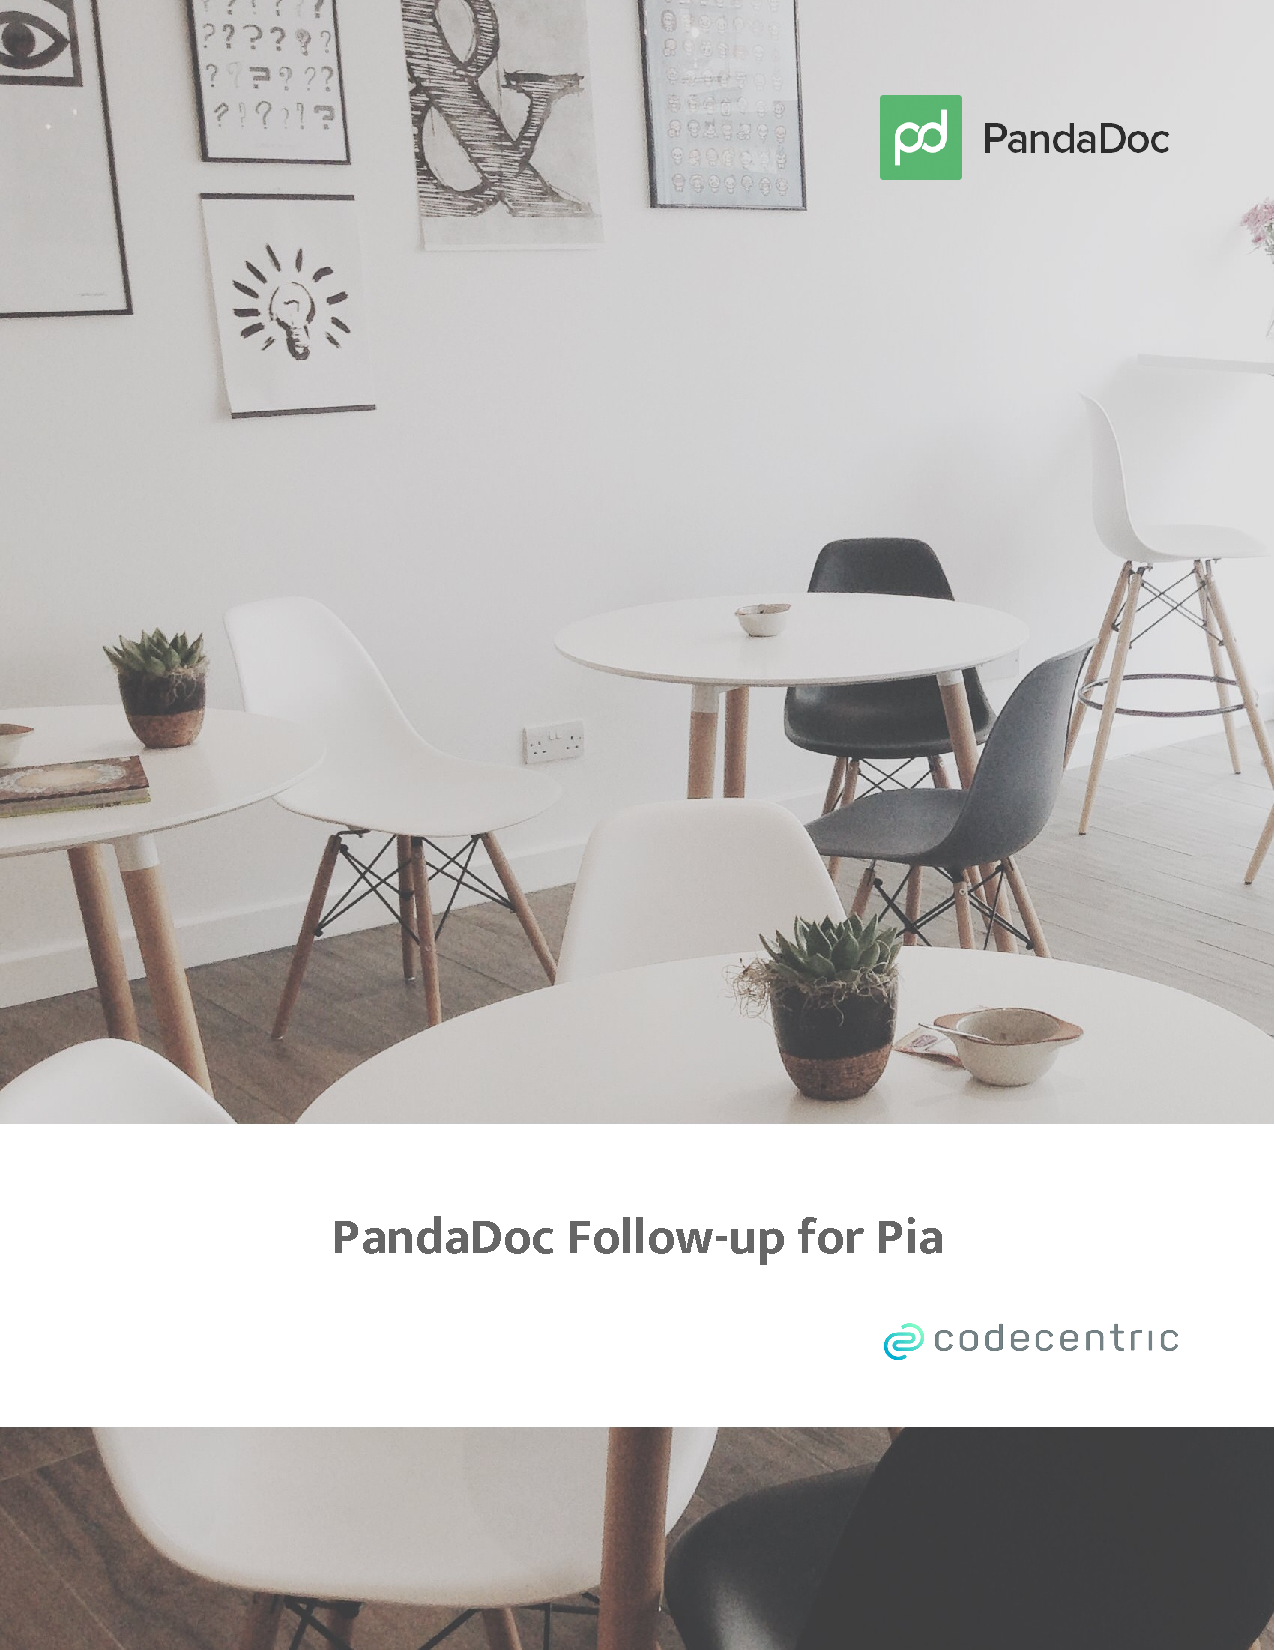
\includepdf[pages=-]{./toolResearch/docs/PandaDocFollow-upforPia.pdf}

\section{Price Information DocuSign} \label{tool:sec:docusignPrice}

\includepdf[pages=-]{./toolResearch/docs/DocuSign.pdf}

\section{Price Information HelloSign} \label{tool:sec:hellosignPrice}

\includepdf[pages=-]{./toolResearch/docs/Codecentric.pdf}

\section{Price Information eSign Live} \label{tool:sec:esignlivePrice}
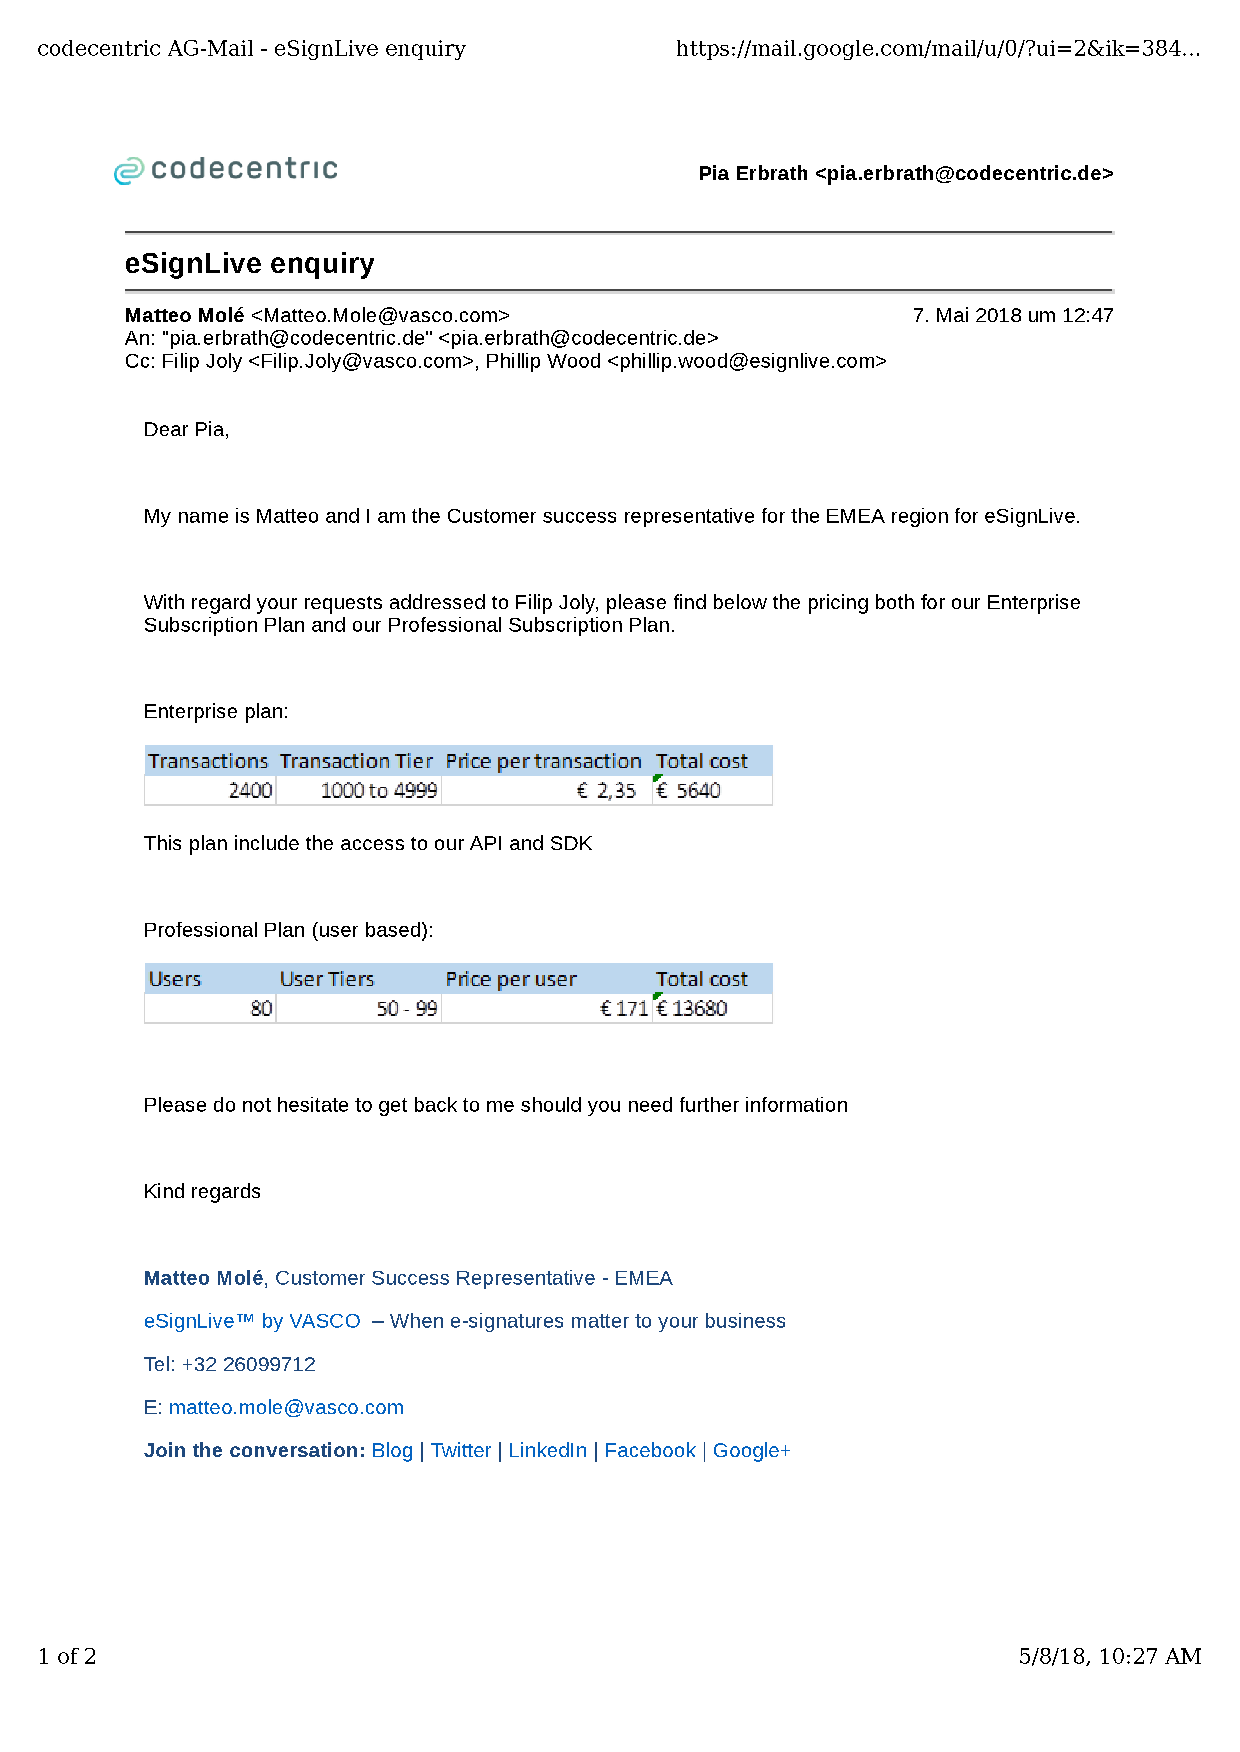
\includepdf[pages=-]{./toolResearch/docs/esignlivePrice.pdf}

\section{Price Information eSignAnyWhere} \label{tool:sec:esignanyPrice}
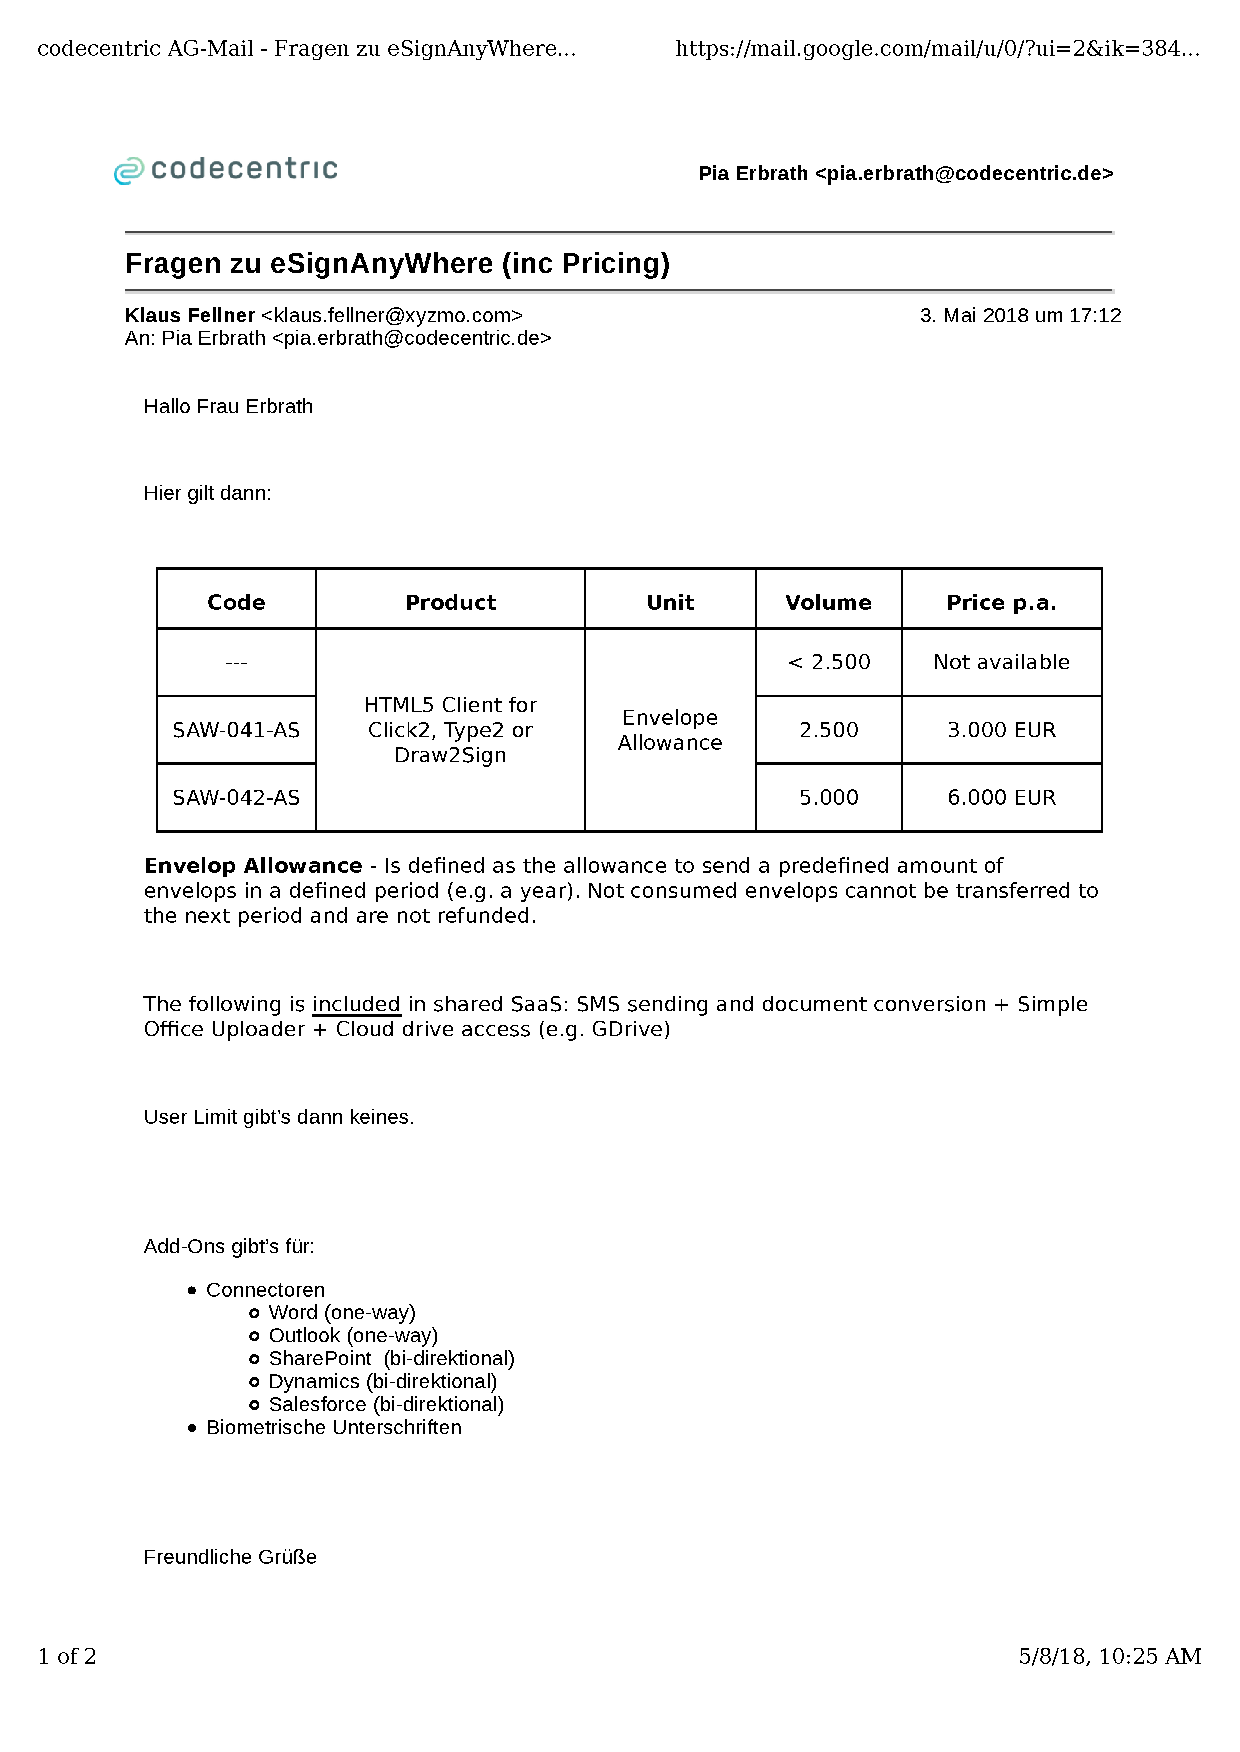
\includepdf[pages=-]{./toolResearch/docs/esignanyPrice.pdf}
%	\input{./docs/PandaDocFollow-upforPia.pdf}
\end{document}